%%%%%%%%%%%%%%%%%%%%%%%%%%%%%%%%%%%%%%%%
% Wenneker Assignment
% LaTeX Template
% Version 2.0 (12/1/2019)
%
% This template originates from:
% http://www.LaTeXTemplates.com
%
% Authors:
% Vel (vel@LaTeXTemplates.com)
% Frits Wenneker
%
% License:
% CC BY-NC-SA 3.0 (http://creativecommons.org/licenses/by-nc-sa/3.0/)
% 
%%%%%%%%%%%%%%%%%%%%%%%%%%%%%%%%%%%%%%%%%

%----------------------------------------------------------------------------------------
%	PACKAGES AND OTHER DOCUMENT CONFIGURATIONS
%----------------------------------------------------------------------------------------

\documentclass[11pt]{scrartcl} % Font size

%%%%%%%%%%%%%%%%%%%%%%%%%%%%%%%%%%%%%%%
% Wenneker Assignment
% Structure Specification File
% Version 2.0 (12/1/2019)
%
% This template originates from:
% http://www.LaTeXTemplates.com
%
% Authors:
% Vel (vel@LaTeXTemplates.com)
% Frits Wenneker
%
% License:
% CC BY-NC-SA 3.0 (http://creativecommons.org/licenses/by-nc-sa/3.0/)
% 
%%%%%%%%%%%%%%%%%%%%%%%%%%%%%%%%%%%%%%%%%

%----------------------------------------------------------------------------------------
%	PACKAGES AND OTHER DOCUMENT CONFIGURATIONS
%----------------------------------------------------------------------------------------
\usepackage{xcolor}   % for \textcolor
\usepackage{comment}

\usepackage{amsmath, amsfonts, amsthm} % Math packages

\usepackage{listings} % Code listings, with syntax highlighting
\usepackage{verbatim} % Directly from txt file

\usepackage[english]{babel} % English language hyphenation
\usepackage{tikz} 
\usepackage{neuralnetwork} 
\usepackage{graphicx} % Required for inserting images
\graphicspath{{Figures/}{./}} % Specifies where to look for included images (trailing slash required)
\usepackage{setspace}  % allows linespacing changes
\usepackage{tabularx} % for tables

\usepackage{booktabs} % Required for better horizontal rules in tables

\numberwithin{equation}{section} % Number equations within sections (i.e. 1.1, 1.2, 2.1, 2.2 instead of 1, 2, 3, 4)
\numberwithin{figure}{section} % Number figures within sections (i.e. 1.1, 1.2, 2.1, 2.2 instead of 1, 2, 3, 4)
\numberwithin{table}{section} % Number tables within sections (i.e. 1.1, 1.2, 2.1, 2.2 instead of 1, 2, 3, 4)

\setlength\parindent{0pt} % Removes all indentation from paragraphs

\usepackage{enumitem} % Required for list customisation
\setlist{noitemsep} % No spacing between list items

%----------------------------------------------------------------------------------------
%	DOCUMENT MARGINS
%----------------------------------------------------------------------------------------

\usepackage{geometry} % Required for adjusting page dimensions and margins

\geometry{
	paper=a4paper, % Paper size, change to letterpaper for US letter size
	top=2.5cm, % Top margin
	bottom=3cm, % Bottom margin
	left=3cm, % Left margin
	right=3cm, % Right margin
	headheight=0.75cm, % Header height
	footskip=1.5cm, % Space from the bottom margin to the baseline of the footer
	headsep=0.75cm, % Space from the top margin to the baseline of the header
	%showframe, % Uncomment to show how the type block is set on the page
}

%----------------------------------------------------------------------------------------
%	FONTS
%----------------------------------------------------------------------------------------

\usepackage[utf8]{inputenc} % Required for inputting international characters
\usepackage[T1]{fontenc} % Use 8-bit encoding

\usepackage{fourier} % Use the Adobe Utopia font for the document

%----------------------------------------------------------------------------------------
%	SECTION TITLES
%----------------------------------------------------------------------------------------

\usepackage{sectsty} % Allows customising section commands

\sectionfont{\vspace{6pt}\centering\normalfont\scshape} % \section{} styling
\subsectionfont{\normalfont\bfseries} % \subsection{} styling
\subsubsectionfont{\normalfont\itshape} % \subsubsection{} styling
\paragraphfont{\normalfont\scshape} % \paragraph{} styling

%----------------------------------------------------------------------------------------
%	HEADERS AND FOOTERS
%----------------------------------------------------------------------------------------

\usepackage{scrlayer-scrpage} % Required for customising headers and footers

\ohead*{} % Right header
\ihead*{} % Left header
\chead*{} % Centre header

\ofoot*{} % Right footer
\ifoot*{} % Left footer
\cfoot*{\pagemark} % Centre footer
 % Include the file specifying the document structure and custom commands
\usepackage{hyperref}

%----------------------------------------------------------------------------------------
%	TITLE SECTION
%----------------------------------------------------------------------------------------

\title{	
	\normalfont\normalsize
	\textsc{Intelligent Robotics, Portland State University}\\ % Your university, school and/or department name(s)
	\vspace{25pt} % Whitespace
	\rule{\linewidth}{0.5pt}\\ % Thin top horizontal rule
	\vspace{20pt} % Whitespace
	{\huge HW4}\\ % The assignment title
	\vspace{4pt} % Whitespace
	{\large Eyebrow Realtime Prediction}\\ % The assignment title
	\vspace{12pt} % Whitespace
	\rule{\linewidth}{2pt}\\ % Thick bottom horizontal rule
	\vspace{12pt} % Whitespace
}

\author{\LARGE Trenton Ruf} % Your name
\date{\normalsize \today} % Today's date (\today) or a custom date

\begin{document}
\maketitle % Print the title
%\renewcommand\thesubsection{\Alph{subsection}}
%\renewcommand\thesubsection{\Roman{subsection}}
%\doublespacing
%\singlespace
%\onehalfspacing
%\setstretch{1.25}

%\begin{doublespace}
%\end{doublespace}

%\vspace*{\fill}
%\clearpage
%\vspace*{\fill}


%\vspace*{\fill}
\renewcommand\thesubsection{\Roman{subsection}}
\section{Overview}
The real-time prediction of my eyebrow state is going to be used to control a model airplane.
This module tests the functionality on a live video feed instead of the saved dataset created in homework 2.
Much of the code is the same between the two homework since a large part of it is capturing and sending images to MediaPipe for face detection, 
and from there cropping my eyebrows out of the image.

\section{Functionality}
If my face is in frame, then there will be text overlaid the user interface with a prediction of my eyebrow state. 
This prediction is made from piping the cropped image of my eyebrows through the tensorflow model created in homework 3. 
The dimensions of the image have to be increased because the model expects a batch of images.
So I send it a batch of 1 image for each prediction.
If my face is not in frame then the overlaid text will read ""Expression: failed".


\section{What is next}
In order to control the plane I will need to make more flight controllers than the altitude hold fuzzy PID created in homework 1.
I will need a bank angle controller, a pitch angle controller, and a rudder turn coordination controller. 
My plan is to create experimental controllers for each of these. 
Potentially utilizing genetic, machine learning, reinforcement learning algorithms. 
I will also need to create my own ROS messages to enable/disable each and to adjust their setpoints. 
A ROS action server will be made to send commands to each controller based on my eyebrow state.

\begin{figure}[ht!] % [h] forces the figure to be output where it is defined in the code (it suppresses floating)
	\centering
	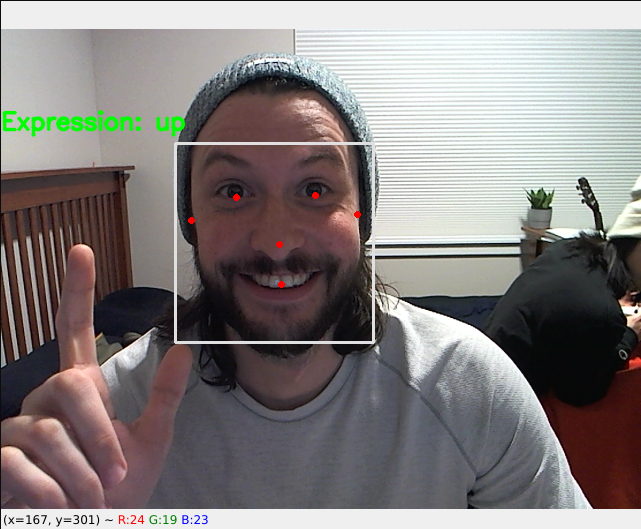
\includegraphics[width=0.49\columnwidth]{figures/up} 
	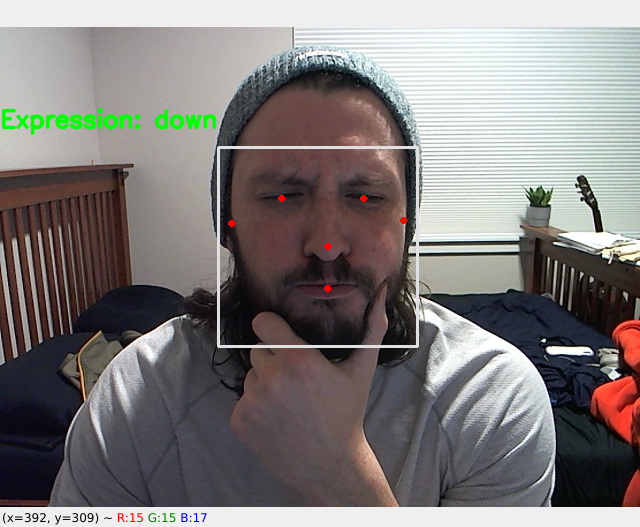
\includegraphics[width=0.49\columnwidth]{figures/down} 
	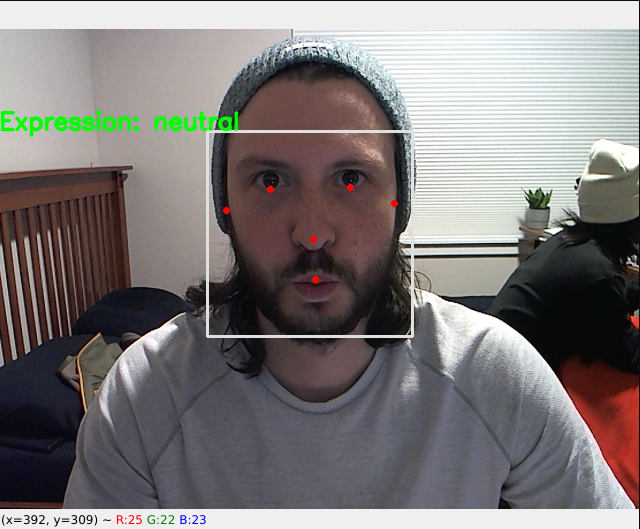
\includegraphics[width=0.49\columnwidth]{figures/neutral} 
	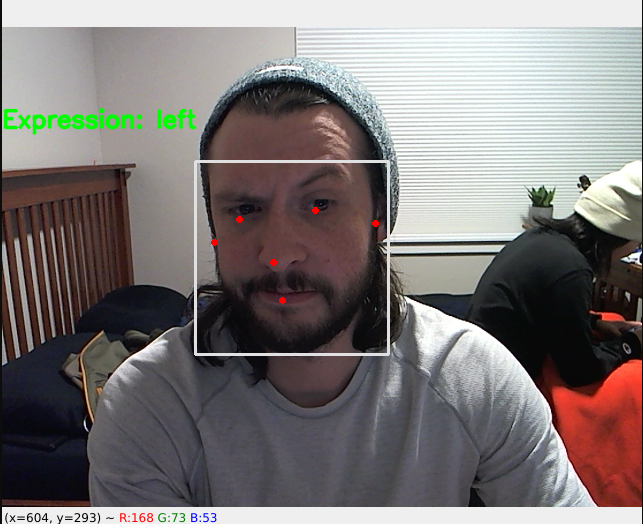
\includegraphics[width=0.49\columnwidth]{figures/left} 
	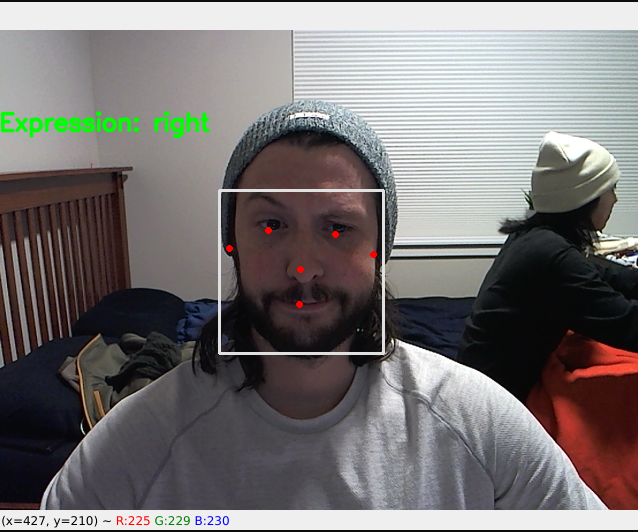
\includegraphics[width=0.49\columnwidth]{figures/right} 
	\caption{Example of the user interface during all eyebrow states.}
\end{figure}

\clearpage
\section{code}

All files related to this project can be found at: 

\url{https://github.com/Trenton-Ruf/Intelligent_Robotics}

\lstinputlisting[
	caption= faceTest.py, % Caption above the listing
	%label=lst:test, % Label for referencing this listing
	language=Python, % Use Perl functions/syntax highlighting
	frame=single, % Frame around the code listing
	breaklines=true,
	postbreak=\mbox{\textcolor{red}{$\hookrightarrow$}\space},	
	showstringspaces=false, % Don't put marks in string spaces
	numbers=left, % Line numbers on left
	numberstyle=\tiny, % Line numbers styling
	basicstyle=\footnotesize
	]{../../../faceCNN/faceTest.py}

\end{document}

